%% 
%% Copyright 2007, 2008, 2009 Elsevier Ltd
%% 
%% This file is part of the 'Elsarticle Bundle'.
%% ---------------------------------------------
%% 
%% It may be distributed under the conditions of the LaTeX Project Public
%% License, either version 1.2 of this license or (at your option) any
%% later version.  The latest version of this license is in
%%    http://www.latex-project.org/lppl.txt
%% and version 1.2 or later is part of all distributions of LaTeX
%% version 1999/12/01 or later.
%% 
%% The list of all files belonging to the 'Elsarticle Bundle' is
%% given in the file `manifest.txt'.
%% 
%% Template article for Elsevier's document class `elsarticle'
%% with harvard style bibliographic references
%% SP 2008/03/01

%\documentclass[preprint,12pt,authoryear]{elsarticle}  %default in the template
%\documentclass[preprint,10pt,authoryear]{elsarticle}

%% Use the option review to obtain double line spacing
%% \documentclass[authoryear,preprint,review,12pt]{elsarticle}

%% Use the options 1p,twocolumn; 3p; 3p,twocolumn; 5p; or 5p,twocolumn
%% for a journal layout:
%% \documentclass[final,1p,times,authoryear]{elsarticle}
%% \documentclass[final,1p,times,twocolumn,authoryear]{elsarticle}
 \documentclass[final,3p,times,authoryear]{elsarticle}
%% \documentclass[final,3p,times,twocolumn,authoryear]{elsarticle}
%% \documentclass[final,5p,times,authoryear]{elsarticle}
%% \documentclass[final,5p,times,twocolumn,authoryear]{elsarticle}

%% For including figures, graphicx.sty has been loaded in
%% elsarticle.cls. If you prefer to use the old commands
%% please give \usepackage{epsfig}

%% The amssymb package provides various useful mathematical symbols
\usepackage{amssymb}
%% The amsthm package provides extended theorem environments
 \usepackage{amsthm}
 \usepackage{amsmath}
 \usepackage{color}
 \usepackage{amsmath}
\usepackage{siunitx}


\usepackage{framed} % Framing content
\usepackage{multicol} % Multiple columns environment
\usepackage{nomencl} % Nomenclature package
\makenomenclature
%\setlength{\nomitemsep}{-\parskip} % Baseline skip between items
\setlength{\nomitemsep}{0.01cm}
\renewcommand*\nompreamble{\begin{multicols}{2}}
\renewcommand*\nompostamble{\end{multicols}}
\newcommand{\degreeC}{\ensuremath{^\circ}C }

\usepackage[nonumberlist]{glossaries}
%\makeglossaries 

\usepackage{dirtree}

%% The lineno packages adds line numbers. Start line numbering with
%% \begin{linenumbers}, end it with \end{linenumbers}. Or switch it on
%% for the whole article with \linenumbers.
%% \usepackage{lineno}

\journal{TBD}

 

\begin{document}




\begin{frontmatter}

%% Title, authors and addresses

%% use the tnoteref command within \title for footnotes;
%% use the tnotetext command for theassociated footnote;
%% use the fnref command within \author or \address for footnotes;
%% use the fntext command for theassociated footnote;
%% use the corref command within \author for corresponding author footnotes;
%% use the cortext command for theassociated footnote;
%% use the ead command for the email address,
%% and the form \ead[url] for the home page:
%% \title{Title\tnoteref{label1}}
%% \tnotetext[label1]{}
%% \author{Name\corref{cor1}\fnref{label2}}
%% \ead{email address}
%% \ead[url]{home page}
%% \fntext[label2]{}
%% \cortext[cor1]{}
%% \address{Address\fnref{label3}}
%% \fntext[label3]{}

\title{Melbourne Google Street View imagery dataset} 




%% use optional labels to link authors explicitly to addresses:
\author[melb]{Kerry A. Nice\corref{cor1}\tnoteref{t1}}
\ead{kerry.nice@unimelb.edu.au}
\author[melb]{Jasper S. Wijnands\tnoteref{t1}}
\address[melb]{Transport, Health, and Urban Design Hub, Faculty of Architecture, Building, and Planning, University of Melbourne, Victoria 3010, Australia}
\cortext[cor1]{Principal corresponding author}
%\cortext[cor2]{First two authors contributed equally}
\tnotetext[t1]{First two authors contributed equally}


\begin{abstract}


This is the abstract.
\end{abstract}

\begin{keyword}
keyword1

\end{keyword}

\end{frontmatter}

% not available 2339092
% total found 4473991
% total locations 1118534



\section{Introduction}\label{sec:introduction}
The Transport, Health, and Urban Design Hub has undertaken a number of studies (CITE TO THEM) requiring large amounts of Google Street View imagery \citep{GoogleMaps2017b}. These images were used in training neural networks to classify urban typologies and a number of other uses. The purpose of this dataset is two-fold, namely (i) providing transparency and replicability of results in the papers mentioned above and (ii) facilitating innovative academic research using Google's street view imagery. The dataset is well curated and can be used for academic, non-commercial research, in accordance with Google's terms of service.

The dataset itself consists of Google Street View imagery for 1.1 million locations in the Greater Melbourne area in Australia. Four images for each location was sampled, with a field of view of 90 degrees and with headings of 0, 90, 180, and 270 degrees. Collected in March 2018.

\section{How the data was collected}\label{sec:create}
In order to efficiently sample data for the Greater Melbourne area, as well as avoid imagery that is not available or that was of indoor locations, the imagery locations were determined by using the road network of Melbourne. Using the AURIN portal \citep{Aurin2018}, the Greater Melbourne area (gccsa\_2016/GMEL) was selected and the PSMA Street Network \citep{PSMA2018} was imported into the project. The PSMA Street Network provides national coverage of the street network at all levels. Roads data covers everything from major highways to walking paths. Using QGIS \citep{QGIS2009}, nodes of the vector lines were extracted from the corresponding shapefile to a new layer. For illustration purposes, an excerpt of this node point layer is provided below:

[replace headers with something more descriptive]
\begin{verbatim}
X, Y, dirn_cd, jrsdctn_id, st_lne_pid, authrty_cd, full_name
144.627419835000012,-37.745644954,2,5639424,VIC5639424,0,GREIGS ROAD
144.616902098999986,-37.746048628,2,5639424,VIC5639424,0,GREIGS ROAD
145.222131428000012,-38.055551055,2,15787712,VIC15787712,0,FOX DRIVE
\end{verbatim}

Using the latitude and longitude locations in this file, Python and the Google Street View API \citep{GoogleMaps2017b} were used to download imagery for the 1.7 million locations. Four images were downloaded for each location, using headings of 0, 90, 180, and 270 degrees. Images for locations where imagery was not available was removed. This brings the total number of available locations to 1.1 million.

The parameters used to download the images are illustrated by the following code excerpt, in which `KEY' is the Google Street View API Key and `number' is the st\_lne\_pid from the PSMA data file (i.e. VIC5639424):

\begin{verbatim}
BUFFER_AREA = 22
IMG_SIZE = 256
url='https://maps.googleapis.com/maps/api/streetview?&size=' + str(IMG_SIZE) +
    'x' + str(IMG_SIZE + 2 * BUFFER_AREA) + '&location=' + str(Lat) +
    ',' + str(Lon) + '&fov=90&heading=' + str(heading) +'&pitch=0&key=' + KEY         
filename = os.path.join(output_dir, '{}_{}_{}_{}.jpg'.format(number, lat, lon,heading))
#image is cropped to remove Google logo for research purposes
w, h = im.size
im.crop((0, BUFFER_AREA, w, h-BUFFER_AREA)).save(filename)
\end{verbatim}

The image dataset described here has been prepared for usage in combination with frequently used neural network architectures (e.g., Inception v2, ...., etc.). As such, the resolution of each image is 256x256 pixels (while the initial download of the image was at a 256x300 resolution). For deep learning purposes, the bottom portions of the images were cropped from 256x300 to 256x256 to remove any superfluous visual information (namely, the Google logo) that would impact neural network training. Hence, when using images from this dataset in academic publications, care should be taken to provide proper attribution to Google.

The four images for each location are saved in the directory structure:

\dirtree{%
.1 Data.
.2 MelbourneStreetView.
.3 000.
.3 090.
.3 180.
.3 270.
}



\section{Description of the data}\label{sec:description}

The dataset contains 4,473,991 images (JPEG 256x256 256x256+0+0 8-bit DirectClass 14.1KB 0.000u 0:00.000) of Google Street View from 1,118,534 locations. Images for each of the four headings (0, 90, 180, and 270 degrees) are saved in the four subdirectories described above. 

Each of the files follow the naming convention LocationNumber\_Latitude\_Longitude\_Heading.jpg (i.e. VIC9984261\_-37.683250063\_145.05143251199999\_90.jpg).

Sample images for -37.932723004,145.032732984 in the four heading directions are shown in Figure \ref{fig:sample}. Total coverage of this dataset is shown in Figure \ref{fig:coverage}.

\begin{figure}[!htbp]
\includegraphics[scale=0.4]{images/{VIC17199075_-37.932723004_145.032732984_0}.jpg} 
\includegraphics[scale=0.4]{images/{VIC17199075_-37.932723004_145.032732984_90}.jpg} 
\includegraphics[scale=0.4]{images/{VIC17199075_-37.932723004_145.032732984_180}.jpg} 
\includegraphics[scale=0.4]{images/{VIC17199075_-37.932723004_145.032732984_270}.jpg} 
\caption{Sample Google Street View imagery for VIC17199075, -37.932723004, 145.032732984 headings 0, 90, 180, and 270 degrees.}    
 \label{fig:sample}  
\end{figure} 


\begin{figure}[!htbp]
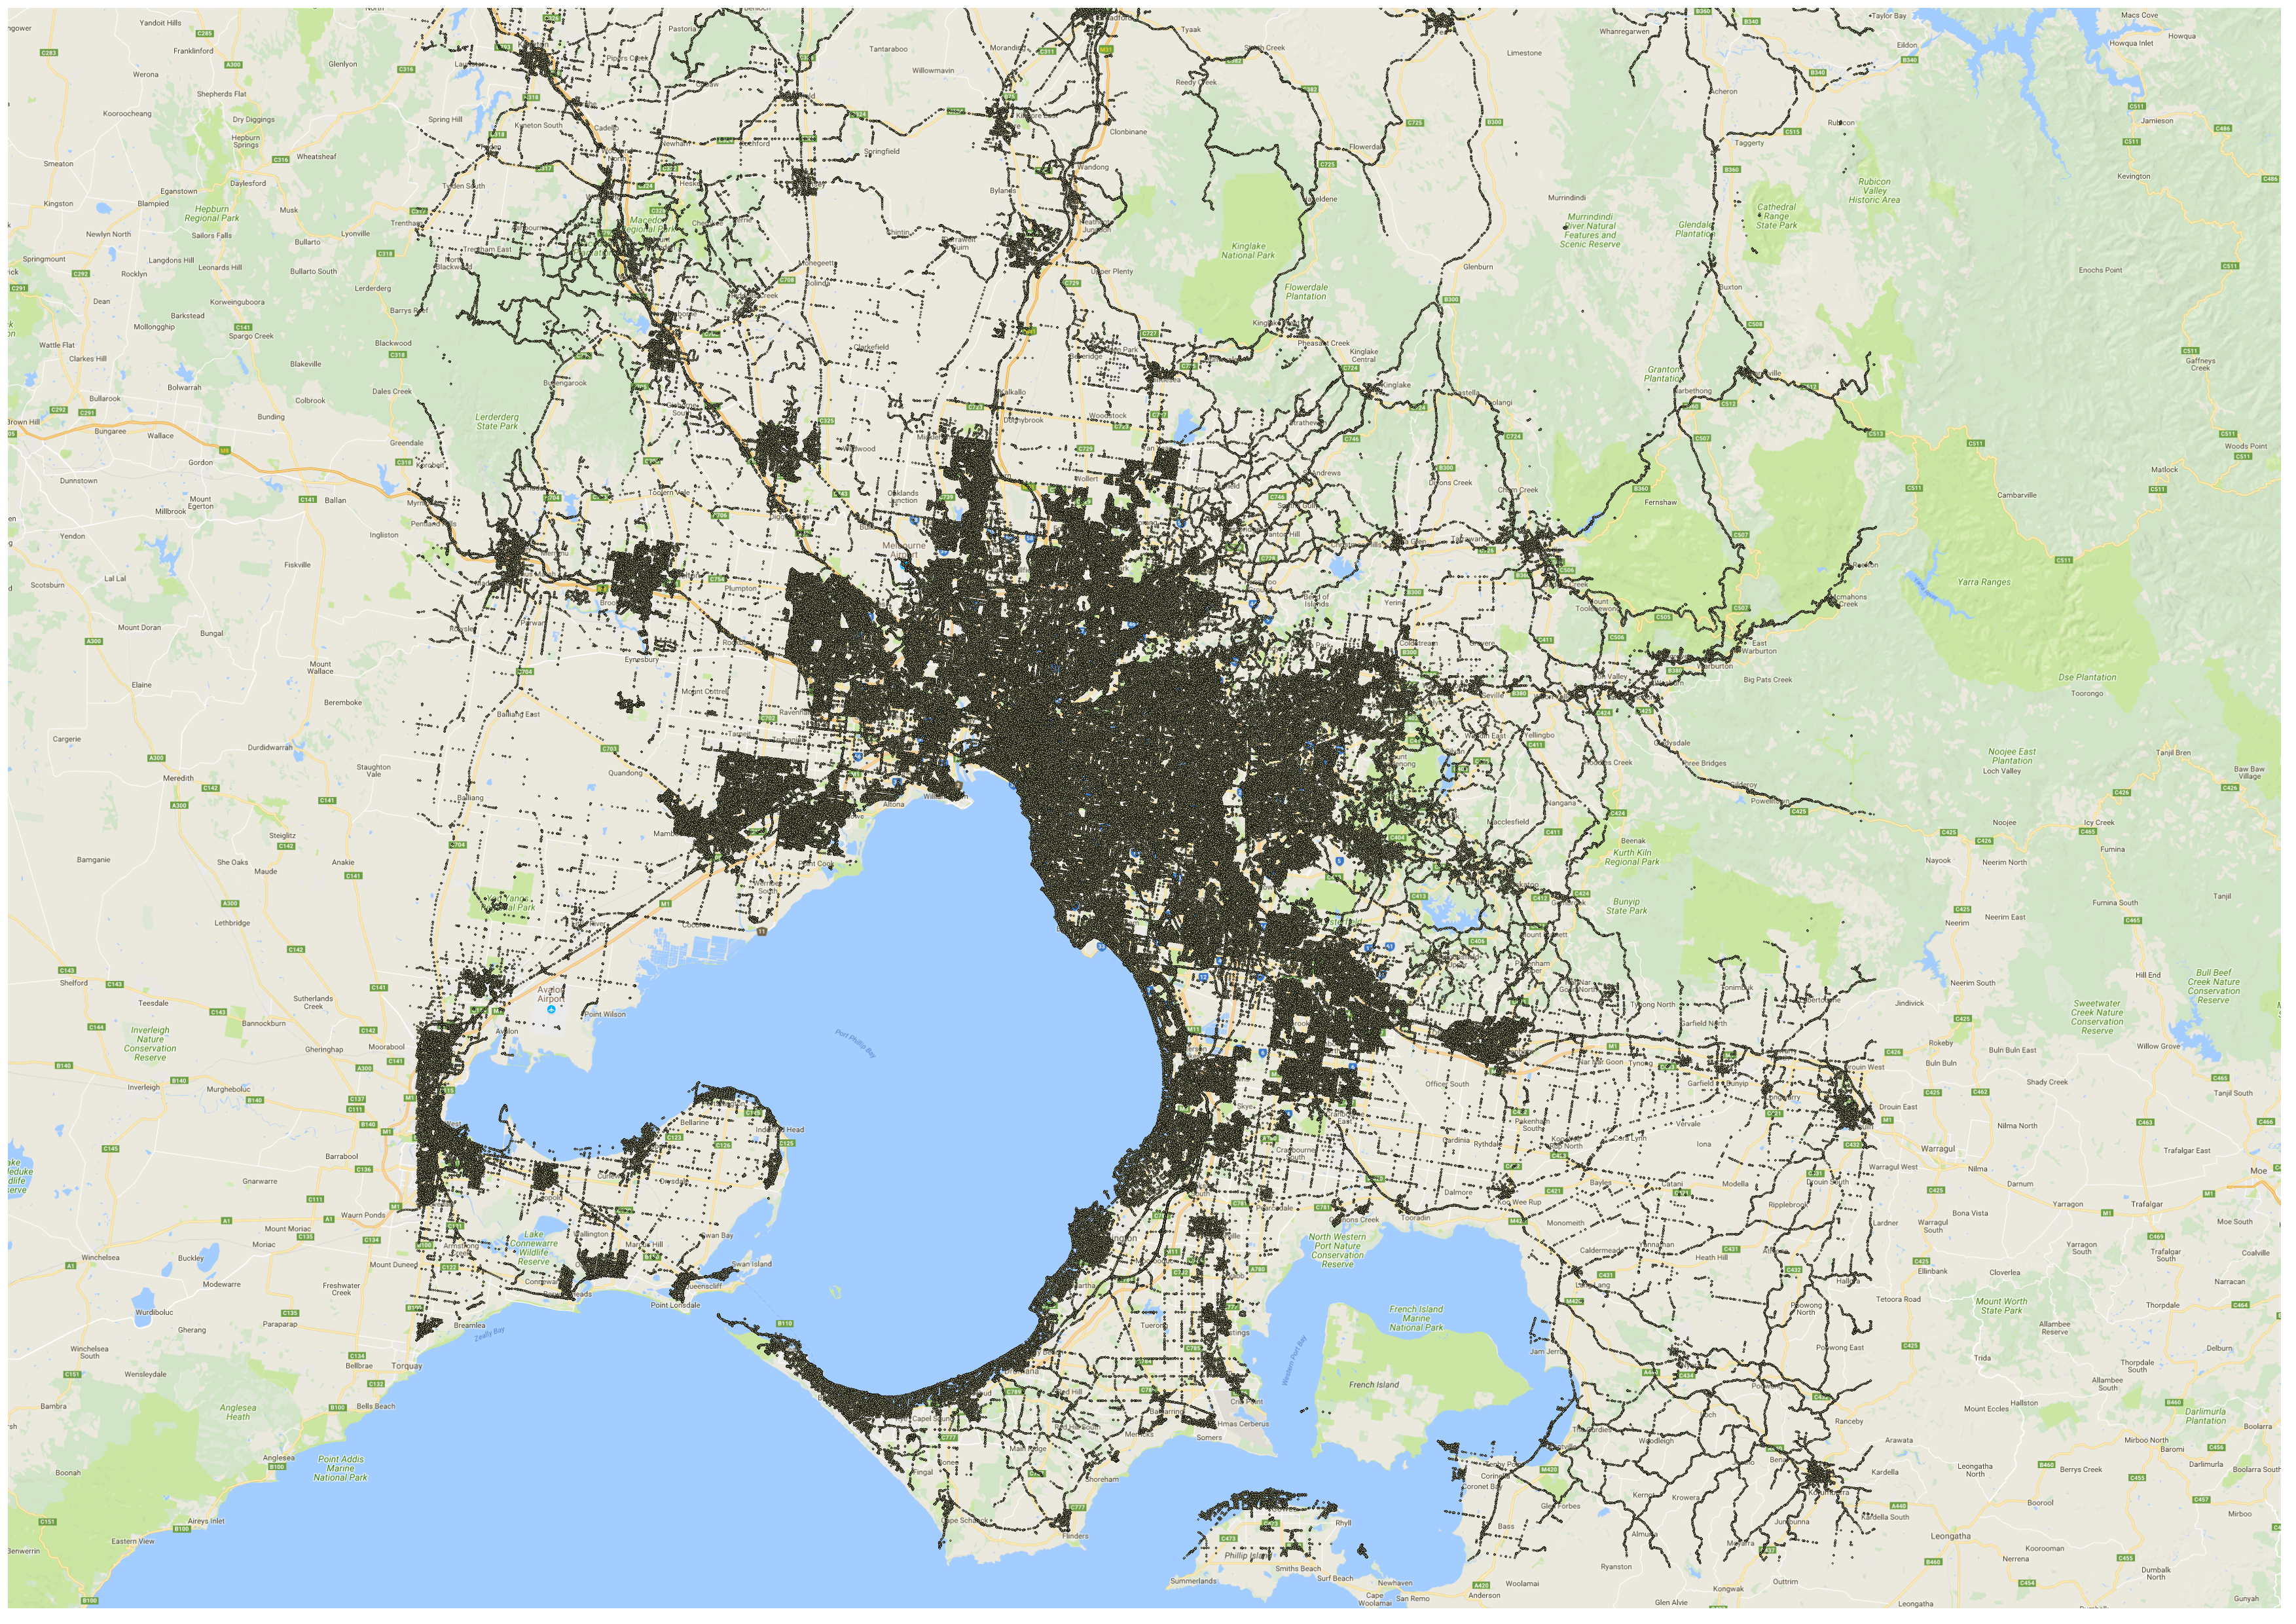
\includegraphics[scale=0.8,trim = 50mm 0mm 50mm 0mm, clip]{images/CoverageOfImagery.png} 
\caption{Coverage of Google Street View imagery.}    
 \label{fig:coverage}  
\end{figure} 




\section*{References}\label{sec:ref}
%% If you have bibdatabase file and want bibtex to generate the
%% bibitems, please use
%%
  \bibliographystyle{elsarticle-harv} 
  \bibliography{library}

%% else use the following coding to input the bibitems directly in the
%% TeX file.

\begin{thebibliography}{00}

%% \bibitem[Author(year)]{label}
%% Text of bibliographic item

\bibitem[ ()]{}

\end{thebibliography}


%% The Appendices part is started with the command \appendix;
%% appendix sections are then done as normal sections
\appendix
\setcounter{table}{0}
\renewcommand{\thetable}{A\arabic{table}}

\section{Obtaining the data}                           
The dataset is available at http://doi.org/XXXXX. It is a XX format file and size X gb. It can be verified with the MD5sum

XXXXXXXXXXXXXXXX

The data is published under XXX licence. If you use this dataset, please cite this paper.

The archive file contains all the images as jpg files. A csv file also links image names, lat/lon locations, location number, and street name.




\end{document}

\endinput
%%
%% End of file `elsarticle-template-harv.tex'.
